\subsubsection{} \textit{RSA} шифровка и расшифровка.
\label{sec:eng:performance:rsaenc}

Метод \texttt{rsaEncrypt} необходим для зашифровки данных при помощи алгоритма \textit{RSA}, а метод \texttt{rsaDecrypt} -- для расшифровки данных, зашифрованных при помощи \textit{RSA}. На рисунках \ref{sec:eng:performance:rsaenc:enc} и \ref{sec:eng:performance:rsaenc:dec} результаты измерений генерации \textit{RSA} и \textit{AES} ключей соответственно.

\begin{figure}[h]
\centering
\begin{minipage}{.5\textwidth}
  \centering
  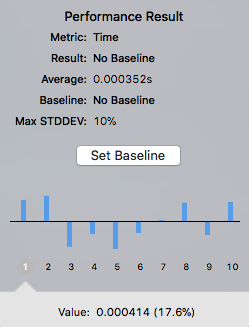
\includegraphics[width=.8\linewidth]{inc/img/perf/testRSAEncryptPerformance.png}
  \captionof{figure}{Результаты замеров шифровки при помощи RSA}
  \label{sec:eng:performance:rsaenc:enc}
\end{minipage}%
\begin{minipage}{.5\textwidth}
  \centering
  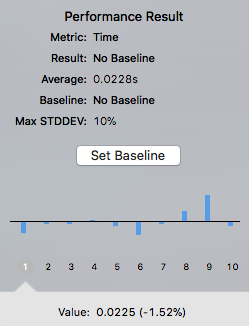
\includegraphics[width=.8\linewidth]{inc/img/perf/testRSADecryptPerformance.png}
  \captionof{figure}{Результаты замеров дешифровки при помощи RSA}
  \label{sec:eng:performance:rsaenc:dec}
\end{minipage}
\end{figure}